\documentclass[11pt]{article}
\usepackage{v-test-paper}
\def\TITLE{Rotation}
\usepackage{enumitem}
\usepackage[export]{adjustbox}


\title{\textsc{\TITLE}}
% \date{February 27, 2024}
\date{Day-10}
\usepackage[none]{hyphenat}
\usetikzlibrary{mindmap}
\usetikzlibrary {patterns,patterns.meta} 

\newcommand{\itemstared}{\refstepcounter{enumi}\item[$^\star$\theenumi.]}
\usetikzlibrary{matrix,  positioning, patterns, backgrounds}
% \renewcommand{\ans}{\quad}
% \renewcommand{\ansint}[1]{\underline{\hspace{2cm}}}


\tikzstyle{root} = [rectangle, rounded corners, 
minimum width=3cm, 
minimum height=0.7cm,
text centered, 
draw, 
font=\scshape,
]
\tikzstyle{child} = [rectangle, rounded corners, 
inner sep=2mm,
text centered, 
draw, 
font=\itshape,
text width=3.25cm,
]

\tikzstyle{child-branch} = [
    rectangle, 
    rounded corners, 
    inner sep=2mm,
    text centered, 
    draw, 
    font=\itshape,
    text width=2.75cm,
]
\tikzstyle{child-stared} = [
    rectangle, 
    rounded corners, 
    inner sep=2mm,
    text centered, 
    draw, 
    font=\itshape,
    text width=2.75cm,
    label={[anchor=north west]north west:*}
]

\tikzstyle{ball}=[
    circle, 
    minimum size=0.5cm, 
    draw, 
    shade,
]



\tikzstyle{arrow} = [thick,->,>=latex]


\begin{document}
\sloppy
\maketitle
% \begin{center}
% \begin{tikzpicture}
    
% \def\root{\TITLE}
% \def\RowOneColOne{Moment Of Inertia}
% \def\RowOneColTwo{Kinematics of a rigid body}
% \def\RowOneColThree{Dynamics of a rigid body}
% \def\RowTwoColOne{Definition Of MOI}
% \def\RowTwoColTwoLeft{Angular Velocity}
% \def\RowTwoColTwoRight{Angular Acceleration}
% \def\RowTwoColThree{Angular Momentum}
% \def\RowThreeColOne{
%     Calculation of MOI
%     \begin{itemize}[itemsep=-2mm, leftmargin=5mm]
%         \item Descrete system of particles
%         \item Contineous destribution of mass
%         \item Parallel axis theorem
%         \item Perpendicular axis theorem
%     \end{itemize}
% }

% \def\RowThreeColTwoLeft{Torque}
% \def\RowThreeColThree{Torque}
% %\def\RowFourColOne{If $\vec{a}_{\textit{COM}}=0$, Conservation of Linear Momentum}
% \def\RowFourColTwoRight{Linear Impluse}
% \def\RowFourColTwoLeft{Variable Mass System(Rocket Propulsion)}

% \matrix [column sep=1mm,row sep=10mm]
% {
% &\node (root) [root] {\root};\\
% \node (row_one_col_one)[child] {\RowOneColOne}; & 
% \node (row_one_col_two)[child] {\RowOneColTwo}; &
% \node (row_one_col_three)[child]{\RowOneColThree};\\
% \node[child](row_two_col_one)at ($(row_one_col_one.south)+(0, 0)$){\RowTwoColOne};& 
% \node[child](row_two_col_two_left)at ($(row_one_col_two.south)+(-2, 0)$){\RowTwoColTwoLeft}; 
% \node[child-branch](row_two_col_two_right) at ($(row_one_col_two.south)+(2, 0)$){\RowTwoColTwoRight};&
% \node(row_two_col_three)[child]{\RowTwoColThree};\\
% \node[child] (row_three_col_one_left) at ($(row_two_col_one.south)+(0, 1)$){\RowThreeColOne};
%  & &
% \node[child-branch] (row_three_col_two_left)at ($(row_two_col_three.south)+(0, 1)$){\RowThreeColTwoLeft};\\
% % &&\\
% % \node[child-stared] (row_four_col_two) at ($(row_three_col_one_left.south)+(-2, 1)$){\RowThreeColTwoLeft};
% % \node[child-stared] (row_four_col_two_right) at ($(row_three_col_one_left.south)+(-5.5, 1)$){\RowFourColTwoRight};\\
% };

% \draw[arrow](root.west)-|(row_one_col_one.north);
% \draw[arrow](root.south)-|(row_one_col_two.north);
% \draw[arrow](root.east)-|(row_one_col_three.north);
% \draw[arrow](row_one_col_one)--(row_two_col_one);
% \draw[arrow](row_one_col_one)--(row_two_col_one);
% \draw[arrow](row_one_col_two)--(row_two_col_two_left);
% \draw[arrow](row_one_col_two)--(row_two_col_two_right);
% \draw[arrow](row_one_col_three)--(row_two_col_three);
% \draw[arrow](row_two_col_one)--(row_three_col_one_left);
% \draw[arrow](row_two_col_three)--(row_three_col_two_left);
% % \draw[arrow](row_two_col_two_right)--(row_three_col_two_left);
% %\draw[arrow](row_three_col_two_left)--(row_four_col_two);
% % \draw[arrow](row_three_col_one_left)--(row_four_col_one);
% \end{tikzpicture}
% \end{center}

\begin{center}
    \textsc{Problems}
\end{center}
\begin{enumerate}

   \item A uniform rod of length $l$ and mass $m$ is suspended on two vertical inextensible strings as shown in figure. Calculate tension $T$ in left string at the instant when right string snaps. 
   
   \begin{center}
    \begin{tikzpicture}[scale=0.8]
    \pic[rotate=180] (ceiling) at (0,0) {frame=7cm};
    \tzcoor(ceiling-center)(O)
    \tzline+[line width=7,line cap=round] ($(O)+(-2.5, -3)$)(5, 0);
    \tzline+($(O)+(-2.5, -3)$)(0, 3);
    \tzline+($(O)+(2.5, -3)$)(0, 3);
    \end{tikzpicture}
    \end{center}
    \begin{tasks}(2)
        \task $\dfrac{mg}{2}$
        \task $mg$
        \task $\dfrac{mg}{4}$\ans
        \task $\dfrac{mg}{8}$
    \end{tasks}

    \item A thin uniform rod of length $l$ and mass $m$ is free to rotate about a smooth pivot which passes through its one end $A$. A point like mass $m$ is shot horizontally at a velocity of $v_0$ towards the lower end of the rod (point $B$). When it hits the rod, it sticks to it. What is the minimum value of $v_0$ required for the rod to reach an angle of $90^\circ$ (horizontal state) ?
    \begin{center}
        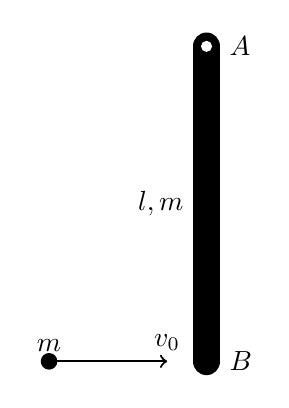
\begin{tikzpicture}
        \draw[thick,line cap=round,line width=10] (0,0) coordinate (a) node[right]{$A$} -- (0,-4) coordinate (b) node[right]{$B$} node[midway, left]{$l,m$};
        \fill[white] (a) circle(2 pt);
        \fill (-2,-4) coordinate (c) circle(3 pt) edge[->, thick] node[at end,above]{$v_0$} ++(1.5,0);
        \node at (c) [above]{$m$};
        \end{tikzpicture}
        \end{center}
    \begin{tasks}(2)
        \task $\sqrt{2gl}$
        \task $\sqrt{3gl}$
        \task $\sqrt{4gl}$\ans
        \task $\sqrt{5gl}$
    \end{tasks}

    \item A  block of mass $m$ moves with a velocity $v_0$ on a smooth horizontal surface. It then passes over a cylinder of radius $R$ and mass $m$, capable of rotating about its own fixed axis through $O$. The block, while passing over, slips on the cylinder. The slipping stops before it loses contact with the cylinder. The block then moves on a similar smooth horizontal surface with a velocity $v$. Find the velocity $v$.
    \begin{center}
        \begin{tikzpicture}
            \pic[xshift=-3.25cm] at (0,0) {frame=3.5cm};
            \pic[xshift=3.25cm] at (0,0) {frame=3.5cm};
            \pic[xshift=-1.5cm,yshift=-1.25cm, rotate=-90] at (0,0) {frame=2.5cm};
            \pic[xshift=1.5cm,yshift=-1.25cm, rotate=90] at (0,0) {frame=2.5cm};
        
        \draw (0,-1) circle[radius=1];
        \draw (-4,0)--++(1.5,0)--++(0,0.5) edge[->] node[at end,above]{$v_0$} ++(1,0) --++(0,0.5)--++(-1.5,0)--cycle ;
        \draw (2.5,0)--++(1.5,0)--++(0,0.5) edge[->] node[at end,above]{$v$} ++(1,0) --++(0,0.5)--++(-1.5,0)--cycle ;
        \draw [->] (0,-1)--([turn]-60:1) node[midway,above]{$R$};
        \fill (0,-1) circle(2pt);
        \end{tikzpicture}
        \end{center}
    \begin{tasks}(2)
        \task $\dfrac{v_0}{3}$
        \task $\dfrac{2v_0}{3}$\ans
        \task $\dfrac{v_0}{4}$
        \task $\dfrac{2v_0}{5}$
    \end{tasks}

    \item A hollow sphere of mass $M$ and radius $R$ filled with water of mass $m$ is rolling on a horizontal surface with linear velocity $v_0$. If water freezes into ice, and the sphere is still rolling on the horizontal surface with linear velocity $v_0$ then find the kinetic energy of the system.
    \begin{center}
        \begin{tikzpicture}
        \pic at (0,0) {frame=5cm};
        \draw (0,1.5) edge[->,thick] node[above]{$R$} ([turn]-60:1.5);
        \fill (0,1.5) circle(2pt);
        \draw[->] (2,1.5)--(3,1.5) node[ above]{$v_0$};
        
        \begin{scope}
           \clip (0,1.5) circle[radius=1.5];
                \foreach  \x in {-1.5,-1.1,...,1.6} \foreach \y in {0,0.5,...,3}
           { \node at (\x,\y) {\small{$-$}};
                \node at (\x + 0.15 ,\y + 0.25) {\small{$-$}};
                   };
        \end{scope}
        
         \draw[very thick] (0,1.5) circle[radius=1.5];
        \end{tikzpicture}
        \end{center}
    \begin{tasks}(2)
        \task $\dfrac{5}{6}Mv_0^2  + \dfrac{7}{10} mv_0^2$\ans
        \task $\dfrac{5}{6}Mv_0^2  + \dfrac{3}{10} mv_0^2$
        \task $\dfrac{5}{6}Mv_0^2  + \dfrac{5}{10} mv_0^2$
        \task $\dfrac{5}{6}Mv_0^2  + \dfrac{4}{10} mv_0^2$
    \end{tasks}

\item A sphere of mass $m$ and radius $R$ rests on sufficiently rough inclined plane in equilibrium as shown in the figure. Find the tension in the string.
\begin{center}
    \begin{tikzpicture}
    \draw (0,0) coordinate (o)--(6,0) coordinate (a);
    \begin{scope}[rotate=30]
    \pic[rotate=120, xshift=1.2cm] at (6,0) {frame=2.4cm};
    \draw (3,2)--(6,2);
    \draw (3,1) coordinate (c) circle[radius=1];
    \draw (0,0)--(6,0) coordinate (b);
    \draw [->] (c)--(3,0) node[midway,right]{$R$};
    \fill  (c) circle(2pt);
    \end{scope}
    \tzanglemark(a)(o)(b){$30^\circ$}(18pt)
    \end{tikzpicture}
    \end{center}
\begin{tasks}(2)
    \task $\dfrac{mg}{2}$
    \task $\dfrac{mg}{3}$
    \task $\dfrac{mg}{4}$\ans
    \task $\dfrac{mg}{5}$
\end{tasks}

\item A rotating ball hits a rough horizontal plane with a vertical velocity $v$ and angular velocity $\omega$. Given that the coefficient of friction is $\upmu$ and the vertical component of the velocity after collision is $v/2$, find the angular velocity after the collision.


\begin{center}
\begin{tikzpicture}
\pic at (0,0) {frame=5cm};
\draw (0,1.5) edge[->] node[at end,right]{$v$} (0,-0.6) circle[radius=1.5];
\fill (0,1.5) circle(2pt);
\tzarc [->] (0,1.5)(130:-60:0.7);
\node at (0.7,1.5)[right]{$\omega$};
\end{tikzpicture}
\end{center}



















   \begin{center}
    \textsc{Comprehension Based Questions}
    \end{center}
{\textbf{Passage I[15 to 18]}}\\
A solid sphere of radius $r$ is set into motion on a rough horizontal surface with a linear speed $v_0$ in forward direction and an angular velocity $\omega_0=\dfrac{v_0}{2r}$ in counter-clockwise direction as shown in figure. If coefficient of friction is $\upmu$, then answer the following questions.
\begin{center}
    \begin{tikzpicture}
    \pic at (0,0) {frame=5cm};
    \draw[->] (0,1.5)--(1,1.5) node[ above]{$v_0$};
    \tzarc [->] (0,1.5)(70:165:2);
    \node at (-2.3,1.5){$\omega_0=\dfrac{v_0}{2r}$};
    \draw[->] (0,1.5)--([turn]120:1.5) node[midway, below]{$r$};
    \draw[ultra thick] (0,1.5) node{$\bullet$} circle[radius=1.5];
    \end{tikzpicture}
    \end{center}

    \item Initial angular acceleration of the sphere will be
    \begin{tasks}(4)
        \task $\dfrac{5\upmu g}{2r}$\ans
        \task $\dfrac{3\upmu g}{2r}$
        \task $\dfrac{2\upmu g}{r}$
        \task $\dfrac{5\upmu g}{r}$
    \end{tasks}

    \item The time after which sphere starts pure rolling is
    \begin{tasks}(4)
        \task $\dfrac{2v_0}{3\upmu g}$
        \task $\dfrac{3v_0}{7\upmu g}$\ans
        \task $\dfrac{v_0}{2\upmu g}$
        \task $\dfrac{v_0}{3\upmu g}$
    \end{tasks}


    \begin{center}
        \textsc{Matrix Match Type}
    \end{center}

   
    

\end{enumerate}




% \vspace*{\fill}

% \begin{center}
\texttt{Answer Key}
\begin{multicols}{5}
\begin{enumerate}
\item (b)
\item (a)
\item (b)
\item (c)
\item (d)
\item (a)
\item (b)
\item (c)
\item (a)
\item (a)
\item (b)
\item (a)
\item (b)
\item (a)
\end{enumerate}
\end{multicols}
\end{center}


% % \begin{figure}[h]
% %     \rotatebox{180}{
% %     \begin{minipage}{\textwidth}
% %         \begin{center}
\texttt{Answer Key}
\begin{multicols}{5}
\begin{enumerate}
\item (b)
\item (a)
\item (b)
\item (c)
\item (d)
\item (a)
\item (b)
\item (c)
\item (a)
\item (a)
\item (b)
\item (a)
\item (b)
\item (a)
\end{enumerate}
\end{multicols}
\end{center}

% %     \end{minipage}
% %     }
% %     \end{figure}



\end{document}